\documentclass[12pt]{report}
\usepackage[margin=1in]{geometry}
\usepackage{setspace} % for single/doublespacing commands
\usepackage{graphicx} % including graphics
\usepackage{sectsty} % sexy section headings
\usepackage{pdfpages} % including multipage pdfs
\usepackage[export]{adjustbox} % for graphic frames and center
\usepackage{siunitx}
\usepackage[numbered]{matlab-prettifier} % including matlab w/ syntax highlighting
\usepackage[T1]{fontenc} % prettier matlab font
\usepackage{xfrac} % more legible inline fractions (\sfrac)
\usepackage{lmodern} % font package for above
\usepackage{multicol} % multiple columns
\usepackage[justification=centering]{caption} % figure captions (force centering)
\usepackage{amsmath} % more math symbols and shit
\usepackage{enumitem} % add arguments for enumerate to change style
\usepackage[list=true]{subcaption} % subfigures with list of figure support
\usepackage{multirow}
\usepackage{mathtools}
\usepackage{booktabs}
\usepackage{color}
\usepackage{ulem}
\usepackage{blindtext}
\usepackage[numbers]{natbib}
\usepackage{contour}
\usepackage{tabularx}
\usepackage{circuitikz} % drawing fancy shit
\usepackage{cancel} % arrow and cross math cancel symbol
\usepackage{lineno}
\usepackage{framed}
\usepackage{amssymb} % special math symbols
\usepackage{listings}
\usepackage{array}
\usepackage{BOONDOX-cal} % fancy mathtype script
\usepackage{fancyhdr}
\usepackage{flowchart}
\usepackage{color, colortbl}
\usepackage{tocloft}
\usepackage{url}
\usepackage{etoolbox}
\usepackage{hyperref}

\setlength{\parskip}{\baselineskip}%
\setlength{\parindent}{0pt}%
\setcounter{secnumdepth}{5}
\renewcommand{\bibname}{References}
\sisetup{output-exponent-marker=\ensuremath{\mathrm{e}}}
\newcommand{\PreserveBackslash}[1]{\let\temp=\\#1\let\\=\temp}
\newcolumntype{C}[1]{>{\PreserveBackslash\centering}p{#1}}
\newcolumntype{R}[1]{>{\PreserveBackslash\raggedleft}p{#1}}
\newcolumntype{L}[1]{>{\PreserveBackslash\raggedright}p{#1}}
\lstMakeShortInline[style=Matlab-editor]| % matlab inline escape character
\graphicspath{{images/}}
\renewcommand\thesection{\arabic{section}}
\renewcommand\labelitemi{---}
\lstset{numberstyle=\ttfamily\small\color{gray}}
\renewcommand\linenumberfont{\ttfamily\small\color{gray}}
\setlength\linenumbersep{6mm}
% \hbadness=99999  % or any number >=10000
\apptocmd{\sloppy}{\hbadness 10000\relax}{}{}
% \usetikzlibrary{arrows,calc,patterns,angles,quotes}
% \usetikzlibrary{shapes.geometric}
% \usetikzlibrary{decorations.pathmorphing,decorations.pathreplacing} % for snakes!
% \usetikzlibrary{positioning, circuits.logic.US}
\setlength{\cftbeforetoctitleskip}{-2em}
\newcommand{\Lag}{\mathcal{L}} % lagrangian L

\apptocmd{\sloppy}{\hbadness 10000\relax}{}{}
\setlength{\cftbeforetoctitleskip}{-2em}
\allsectionsfont{\raggedright}
\setlist[enumerate]{wide=0pt, widest=99,
                    leftmargin=\parindent,topsep=0pt,partopsep=0pt,
                    label=\thesubsubsection.\alph*,font=\itshape}
\begin{document}
\normalem
\begin{titlepage}
\flushleft
\doublespacing
\Large
\textsc{Test Document} \\
\normalsize
Trey Dufrene, Zack Johnson, David Orcutt, Alan Wallingford, Ryan Warner
\vfill
\center
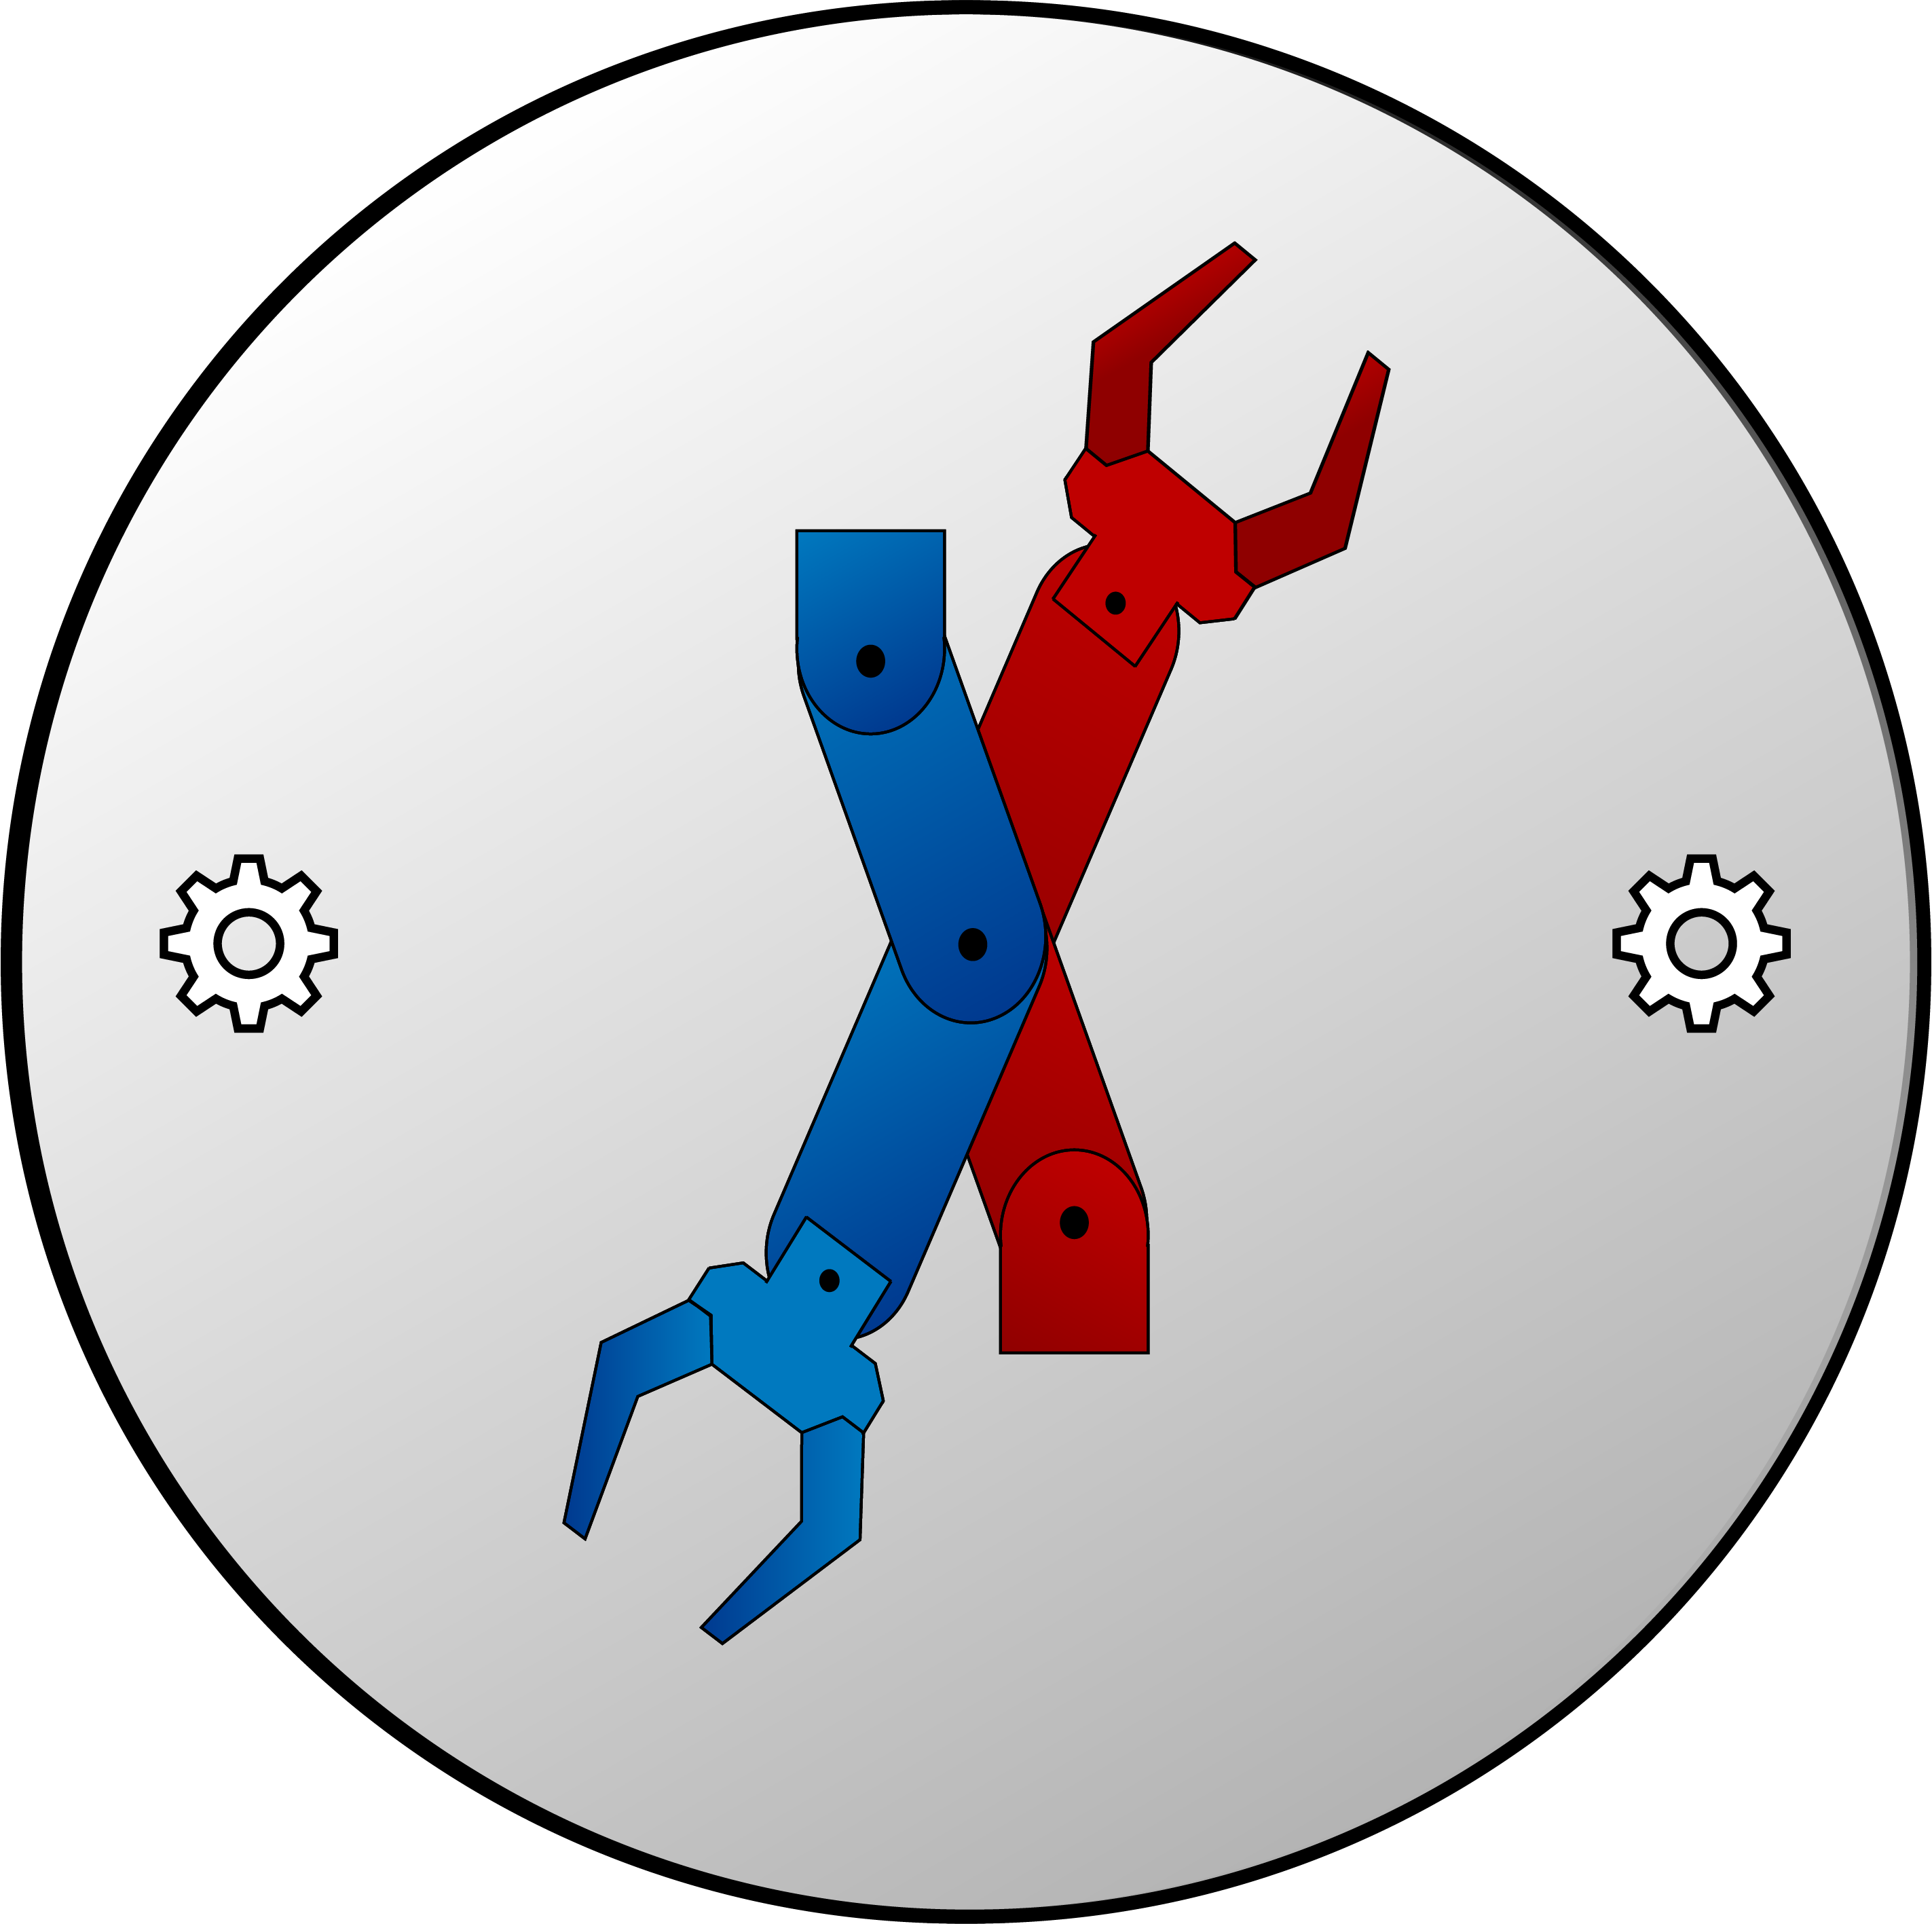
\includegraphics[width=.45\textwidth]{logo}
\vfill
\flushleft
ME 407 \\
Preliminary Design of Robotic Systems \\
Embry-Riddle Aeronautical University \\
\vspace{2ex}
\begin{minipage}[c]{.5\textwidth}
\flushleft

\includegraphics[width=.95\textwidth]{erau}
\end{minipage}%
\begin{minipage}[c]{.5\textwidth}
\flushright

\includegraphics[width=.8\textwidth]{text}
\end{minipage}
\end{titlepage}

\pagenumbering{roman}
% \begin{abstract}
  % Wordy words
% \end{abstract}
{\tableofcontents\let\clearpage\relax\listoffigures\let\clearpage\relax\listoftables}
\clearpage
\newpage

% \section*{List Of Acronyms and Abbreviations}

% \begin{tabular}{rl}
%   $G$~:&Center of gravity of the bar \\
%   $\ell_0$~:& Spring unstretched length  \\
%   $\delta$~:& Spring deflection \\
%   $k$~:& Spring constant \\
%   $h_{b}$~:& Distance to bar ($G$) from datum \\
%   $F_s$~:& Force onto bar due to spring\\
%   $A_{n}$~:& Pin reaction in $\theta$ direction\\
%   $A_{t}$~:& Pin reaction in tangential direction \\
%   $\vec{v}_G$~:& Velocity of bar center of gravity\\
%   $\ddot{\theta}$~:& Angular velocity of spring \\
%   $\ddot{\phi}$~:& Angular velocity of bar\\
%   $\ddot{\ell}_s$~:& Radial acceleration of spring \\
% \end{tabular}
% \normalsize
% \flushleft
% \singlespacing
% \newpage

\pagenumbering{arabic}

\section{Forward Kinematics}
\begin{table}[htp]
  \center
  \caption{DH Table for 6 DOF Manipulator}
  \label{table:dh}
  \begin{tabular}{C{1cm}|C{1.5cm}|C{2cm}|C{1cm}|C{1cm}}
    DH & $d_i$ & $\theta_i$ & $a_i$ & $\alpha_i$ \\ \hline
    1 & $\ell_1$ & $\theta_1$ & 0 & $\sfrac{\pi}{2}$ \\
    2 & $-d$ & $\theta_2$ & $\ell_2$ & 0 \\
    3 & 0 & $\theta_3 + \sfrac{\pi}{2}$ & 0 & $\sfrac{\pi}{2}$ \\
    4 & $\ell_3 + \ell_4$ & $\theta_4$ & 0 & $-\sfrac{\pi}{2}$ \\
    5 & 0 & $\theta_5$ & 0 & $\sfrac{\pi}{2}$ \\
    6 & $\ell_6$ & $\theta_6$ & 0 & 0 \\
  \end{tabular}
\end{table}
Where \(\ell_1 = 22.08\)cm, \(\ell_2 = 25\)cm, \(\ell_3 = 20\)cm, \(\ell_4 = 8\)cm, \(\ell_6 = 5.25\)cm, and \(d = 1\)cm.
\begin{equation}
A = Rot_{z,\theta}~Trans_{z,d}~Trans_{x,a}~Rot_{x,\alpha}
\label{eq:J1}
\end{equation}%
Given an arbitrary homogeneous matrix $T_i^{i-1}$ (computed by matrix multiplication of $A$ matrices $\rightarrow \big[A_1A_2\cdots A_{i-1}A_i\big]$), the orientation vector $\bar{z}_i$ (with respect to $\varphi$, $\theta$ and $\psi$) and the relative joint position (displacement) vector $\bar{o}_i$ (with respect to $x$, $y$, and $z$) can be obtained via the 3$^{rd}$ and 4$^{th}$ columns of the matrix respectively,
as shown in Equation \ref{eq:J2} (given $\beta$ as an arbitrary rotation angle about the $z$-axis).
\begin{equation}
  T_i^{i-1} =
\begin{bmatrix}
  c_{\beta} & -s_{\beta} & z_i^{\varphi} & o_i^x \\
  s_{\beta} & c_{\beta} & z_i^{\theta} & o_i^y \\
  0 & 0 & z_i^{\psi} & o_i^z \\
  0 & 0 & 0 & 1 \\
\end{bmatrix}
\label{eq:J2}
\end{equation}
\begin{minipage}[b]{.5\textwidth}
  \strut\vspace*{-\baselineskip}\newline
\[
A_1 = rotz(\theta_1) ~ transz(\ell_1) ~ rotx(\sfrac{\pi}{2})
\]
\vspace{.25ex}
\[
A_1 =
\begin{bmatrix}
  \cos(\theta_1) & 0 & \sin(\theta_1) & 0 \\
  \sin(\theta_1) & 0 & -\cos(\theta_1) & 0 \\
  0 & 1 & 0 & 22.08 \\
  0 & 0 & 0 & 1 \\
\end{bmatrix}
\]
\end{minipage}%
\begin{minipage}[b]{.5\textwidth}
\strut\vspace*{-\baselineskip}\newline
\[
A_2 = rotz(\theta_2) ~ transz(-d) ~ transx(\ell_2)
\]
\vspace{.25ex}
\[
A_2 =
\begin{bmatrix}
  \cos(\theta_2) & -\sin(\theta_2) & 0 & 25\cos(\theta_2) \\
  \sin(\theta_2) & \cos(\theta_2) & 0 & 25\sin(\theta_2) \\
  0 & 0 & 1 & -1 \\
  0 & 0 & 0 & 1 \\
\end{bmatrix}
\]
\end{minipage}\\
\begin{minipage}[c]{.5\textwidth}
\[
A_3 = rotz(\theta_3 + \sfrac{\pi}{2}) ~ rotx(\sfrac{\pi}{2})
\]
\vspace{.25ex}
\[
A_3 =
\begin{bmatrix}
  \cos(\theta_3 +  \sfrac{\pi}{2}) & 0 & \sin(\theta_3 +  \sfrac{\pi}{2}) & 0 \\
  \sin(\theta_3 +  \sfrac{\pi}{2}) & 0 & -\cos(\theta_3 +  \sfrac{\pi}{2}) & 0 \\
  0 & 1 & 0 & 0 \\
  0 & 0 & 0 & 1 \\
\end{bmatrix}
\]
\end{minipage}%
\begin{minipage}[c]{.5\textwidth}
\[
A_4 = rotz(\theta_4) ~ transz(\ell_3 + \ell_4) ~ rotx(-\sfrac{\pi}{2})
\]
% \vspace{.25ex}
\[
A_4 =
\begin{bmatrix}
  \cos(\theta_4) & 0 & -\sin(\theta_4) & 0 \\
  \sin(\theta_4) & 0 & \cos(\theta_4) & 0 \\
  0 & -1 & 0 & 28 \\
  0 & 0 & 0 & 1 \\
\end{bmatrix}
\]
\vspace{.25ex}
\end{minipage}\\
\begin{minipage}[c]{.5\textwidth}
\[
A_5 = rotz(\theta_5) ~ rotx(\sfrac{\pi}{2})
\]
\vspace{.25ex}
\[
A_5 =
\begin{bmatrix}
  \cos(\theta_5) & 0 & \sin(\theta_5) & 0 \\
  \sin(\theta_5) & 0 & -\cos(\theta_5) & 0 \\
  0 & 1 & 0 & 0 \\
  0 & 0 & 0 & 1 \\
\end{bmatrix}
\]
\end{minipage}%
\begin{minipage}[c]{.5\textwidth}
\[
A_6 = rotz(\theta_6) ~ transz(\ell_6)
\]
\vspace{.5ex}
\[
A_6 =
\begin{bmatrix}
  \cos(\theta_6) & 0 & -\sin(\theta_6) & 0 \\
  \sin(\theta_6) & 0 & \cos(\theta_6) & 0 \\
  0 & 0 & 1 & 5.25 \\
  0 & 0 & 0 & 1 \\
\end{bmatrix}
\]
\vfill\null
\end{minipage}




% A Level:
% \section{}
% B Level:
% \subsection{B Level Heading}
% C Level
% \subsubsection{}

% Example citations:
% \cite{DBLP:journals/corr/JohnsonAL16}
% \cite{DBLP:journals/corr/abs-1803-09820}
% \cite{DBLP:journals/corr/RonnebergerFB15}

% \section{A Level Heading}
% Sample table with tabulated data and reference label
% \begin{table}[htp]
%   \center
%   \caption{DH Table for 6 DOF Manipulator}
%   \label{table:dh}
%   \color{red} bold col headers, table times new roman, 12pt., centered, \color{black} \\
%   \begin{tabular}{C{1cm}|C{1cm}C{2cm}C{1cm}C{1cm}}
%     \textbf{DH} & $d_i$ & $\theta_i$ & $a_i$ & $\alpha_i$ \\ \hline
%     1 & 280 & $q_1 - \pi$ & 0 & $\sfrac{\pi}{2}$ \\
%     2 & 0 & $q_2 + \sfrac{\pi}{2}$ & 210 & 0 \\
%     3 & 0 & $q_3 - \sfrac{\pi}{2}$ & 75 & -$\sfrac{\pi}{2}$ \\
%     4 & 210 & $q_4$ & 0 & $\sfrac{\pi}{2}$ \\
%     5 & 0 & $q_5 - \pi$ & 0 & $\sfrac{\pi}{2}$ \\
%     6 & 70 & $q_6$ & 0 & 0 \\
%   \end{tabular}
% \end{table}
% here is the table reference callout
% \emph{Table \ref{table:dh}} shows the Denavit–Hartenberg parameters for the manipulator.

% Here is a centered mathtype with no number
% $$
% \vec{v}_G =
% \left[\dot{\ell}_s\sin(\theta) + \frac{\ell_b\dot{\phi}\cos(\phi)}{2} +
% \ell_s\dot{\theta}\cos(\theta)\right]\hat{\textrm{\i}} +
% \left[\frac{\ell_b\dot{\phi}\sin(\phi)}{2} -
% \dot{\ell}_s\cos(\theta) + \ell_s\dot{\theta}\sin(\theta)\right]\hat{\textrm{\j}}
% $$

% Here is a centered equation with number and reference label
% \begin{equation}
% \ddot{\theta} = \frac{d}{dt}\left(\frac{\partial\Lag}{\partial\dot{\theta}}\right) -
% \frac{\partial\Lag}{\partial\theta} = \big(Q_{\theta}\big)_{\text{non}}
% \label{eq:lagtheta}
% \end{equation}

% This is some inline mathtype: $u = \frac{1}{2}mv^2$, (notice the fluidity and smaller size than the other mathtype)

% \section{A Level Heading}
% \begin{figure}[h]
%   \centering
%   \includegraphics[width=.75\textwidth]{filename}
%   \caption{Figure with Callouts}
%   \label{fig:figname}
% \end{figure}

% \begin{enumerate}[label=\alph*.]
%   \item Description for callout a
%   \item Description for callout b
% \end{enumerate}

% As seen in \emph{Figure \ref{fig:figname}}

% \newpage
% \bibliographystyle{plain}
% \bibliography{JohnsonAL16,abs-1803-09820,RonnebergerFB15}

% \newpage
% \section*{Acknowledgements \& Attributions}
% \begin{itemize}
%   \item People!
% \end{itemize}
% \newpage

% \newpage
% \appendix
% \renewcommand\thesection{\Roman{section}}
% \renewcommand\thesubsection{\roman{subsection}}
% \section*{Appendix}\label{sec:app}
% Code listing
%\begin{lstlisting}[frame=lines,style=Matlab-editor,basicstyle = \mlttfamily, caption=Example Code
% Code Here
%\end{lstlisting}

% \includepdf[landscape,pages=-]{pdfname}

\end{document}
